\documentclass[tikz,border=2pt]{standalone}
\usepackage{amsmath}
\usetikzlibrary{arrows.meta}
\begin{document}
% Left: prisoner's dilemma stage game v(C,C)=(3,3), v(C,D)=(0,5), v(D,C)=(5,0), v(D,D)=(1,1);
% (D,D) is the unique stage-game Nash equilibrium. Right: if player 2 plays C with probability y,
% player 1 earns 3y from C and 1+4y from D; since 1+4y > 3y for every y, D is strictly dominant.
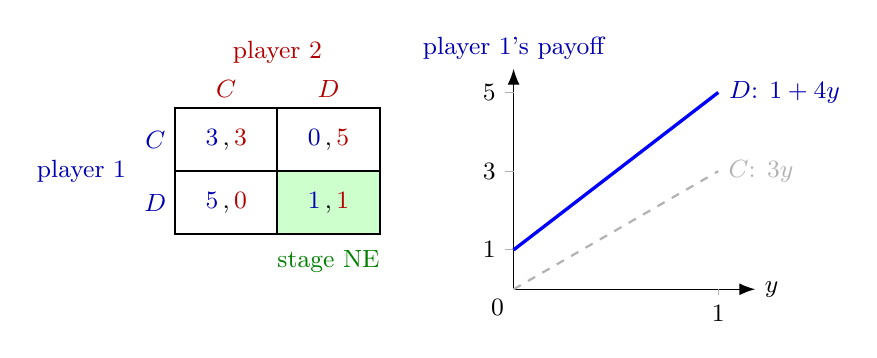
\begin{tikzpicture}[font=\small, >={Latex[length=2mm]}]
  % ---- stage game matrix
  \begin{scope}
    \def\w{1.3} \def\h{0.8}
    \fill[green!20] (\w,-\h) rectangle (2*\w,0);
    \draw[thick] (0,-\h) rectangle (2*\w,\h);
    \draw[thick] (\w,-\h) -- (\w,\h);
    \draw[thick] (0,0) -- (2*\w,0);
    \node[red!70!black] at (0.5*\w,\h+0.25) {$C$};
    \node[red!70!black] at (1.5*\w,\h+0.25) {$D$};
    \node[blue!70!black] at (-0.25,0.5*\h) {$C$};
    \node[blue!70!black] at (-0.25,-0.5*\h) {$D$};
    \node[red!70!black, anchor=south] at (\w,\h+0.45) {player 2};
    \node[blue!70!black, anchor=east] at (-0.5,0) {player 1};
    \node at (0.5*\w,0.5*\h) {\textcolor{blue!70!black}{$3$}\,,\,\textcolor{red!70!black}{$3$}};
    \node at (1.5*\w,0.5*\h) {\textcolor{blue!70!black}{$0$}\,,\,\textcolor{red!70!black}{$5$}};
    \node at (0.5*\w,-0.5*\h) {\textcolor{blue!70!black}{$5$}\,,\,\textcolor{red!70!black}{$0$}};
    \node at (1.5*\w,-0.5*\h) {\textcolor{blue!70!black}{$1$}\,,\,\textcolor{red!70!black}{$1$}};
    \node[green!50!black, anchor=north] at (1.5*\w,-\h-0.08) {stage NE};
  \end{scope}
  % ---- player 1's payoffs from C and D against y
  \begin{scope}[xshift=4.3cm, yshift=-1.5cm, x=2.6cm, y=0.5cm]
    \draw[->] (0,0) -- (1.18,0) node[right] {$y$};
    \draw[->] (0,0) -- (0,5.6) node[above, blue!70!black] {player 1's payoff};
    \foreach \t in {1,3,5} {\draw[gray!60] (0,\t) -- (-0.04,\t) node[left, black] {$\t$};}
    \draw[gray!60] (1,0) -- (1,-0.15) node[below, black] {$1$};
    \node[below left] at (0,0) {$0$};
    \draw[gray!60, thick, dashed] (0,0) -- (1,3) node[right] {$C$: $3y$};
    \draw[blue, very thick] (0,1) -- (1,5) node[right, blue!70!black] {$D$: $1+4y$};
  \end{scope}
\end{tikzpicture}
\end{document}
